\documentclass[handout,t]{beamer}
% Para alterar a linguagem do documento
\usepackage[english,russian]{babel}
% Para aceitar caracteres especias deretamente do teclado
\usepackage[utf8]{inputenc}
% Para seguir as normas da ABNT de citacao e referencias
\usepackage[alf]{abntex2cite}
% Para incluir figuras
\usepackage{graphicx}
% Para melhor ajuste da posisao das figuras
\usepackage{float}
% Para ajustar as dimensoes do layout da pagina
\usepackage{geometry}
% Para formatar estrutura e informacoes de formulas matematicas
\usepackage{amsmath}
% Para incluir simbolos especiais em formulas matematicas
\usepackage{amssymb}
% Para incluir links nas referencias
\usepackage{url}
% Para incluir paginas de documentos .pdf externos
\usepackage{pgfpages}
% Para ajustar o estilo dos contadores
\usepackage{enumerate}
% Para modificar a cor do texto
\usepackage{color}
% Para incluir condicoes
\usepackage{ifthen}
% Para colocar legendas em algo que nao e float
\usepackage{capt-of}
% Para definir o tema do slide
\usetheme{Frankfurt}
% Para difinir cores e background
\usepackage{floatflt}
\usepackage{wrapfig}
\usepackage{nccfloats}
\usepackage{setspace} 
\usecolortheme{ufrn} 
% Para numerar as figuras
\setbeamertemplate{caption}[numbered]
\usepackage{graphicx}
\graphicspath{{pictures/}}
\DeclareGraphicsExtensions{.pdf,.png,.jpg}
\usepackage{graphicx}
\usepackage{multimedia}
\usepackage{hyperref}
% Titl
\title[Leidenfrost Effect]{Dynamic Leidenfrost Effect:\\
Relevant Time and Length Scales
	}
% Data
\date{
	10.06.2022\\
	\vspace{0.2cm}
	10.06.2022}
% Autores
\author[Viktor Krayushkin]{
	Autor \inst{1}\\
	\vspace{0.2cm}
	Autor \inst{2}\\
	\vspace{0.2cm}}
% Instituto
\institute[INSTITUTO]{
	\inst{1}%
	Krayushkin\ Viktor\\
	\vspace{0.2cm}
	\inst{2}%
	Дьяконов Максим\\
	\vspace{0.2cm}
	b04-108\\
	\vspace{0.2cm}
	\inst{1}%
kraiushkin.vp@phystech.edu\\
\inst{2}%
dyakonov.ma@phystech.edu}
\begin{document}
% list of contents
\frame{\titlepage}
\section[]{}
\begin{frame}{list of contents}
	\tableofcontents
\end{frame}
% Introducao
\section{Introduction}
\begin{frame}{Introduction}
\vspace{0.25cm}
\begin{block}{Каким образом находится Leidenfrost Point?}
    Эксеперементальное определение точки Leidenfrost Point с помощью графика зависимости времени жизни капли
    (дистилированной воды) от температуры разогретой поверхности.
\end{block}
    \vspace{0.25cm}
\begin{itemize}
\item На первом этапе теоретически определяем значения температуру of Leidenfrost Point для воды.
\vspace{0.25cm}
\item Вторым этапом находим эксперементальные значения.
\vspace{0.25cm}
    \item Третьим этапом строим график по собранным и обработанным данным.
    \vspace{0.25cm}
\end{itemize}
\end{frame}
\begin{frame}{В чём практическая польза в исследованиях тепературы Leidenfrost Point?}
\vspace{0.30cm}
\begin{block}{}
\textsl{\Large Начало стабильного плёночного кипения играет важную роль в следующих физических процессах:}
\end{block}
 \vspace{0.25cm}
\renewcommand{\labelenumii}{\arabic{enumi}.\arabic{enumii}.}
\begin{enumerate} 
\large
    \item 

 переходном поведении воды 
 \vspace{0.15cm}
 \item органическом охлаждении ядерных реакторов 
 \vspace{0.15cm}
 \item поведении криогенных устройств 
 \vspace{0.15cm}
 \item охлаждении ракетных форсунок.\\   
 \vspace{0.15cm}
\end{enumerate}
\end{frame}
% Metodologia
\section{Theoretical background}
\begin{frame}{Первые уравнения,начало развития}
\begin{block}{Модель}
Прогнозирование температуры поверхности стенки в начале стабильного плёночного кипения.
\end{block}
\vspace{0.10cm}
 У модели две особенности:
  \vspace{0.05cm}
 \begin{itemize}
\item первое, то что температура стенки, при которой начинается стабильное плёночное кипение - это foam limit (предел пены), то есть максимальная температура, до которой жидкость может быть перегрета.
 \vspace{0.05cm}
\item второе, то что предел пенообразования можно вычислить и довольно точно из уравнения Ван-дер-Ваальса. Экспериментальные  данные о начале стабильного кипения плёнки хорошо согласуются с температурами стенки, предсказанными этой моделью. 
\end{itemize}
\end{frame}
\begin{frame}{вывод формулы}
\begin{equation}
p^{'}=\frac{8T^{'}}{3\left(\n\upsilon'-1/3\right)}-\frac{3}{\left(\upsilon'\right)^2},
\label{eq:1}
\end{equation}
\[ \quad   p^{'}=\frac{p}{p_{c}},\ \quad \quad \upsilon^{'}=\frac{\upsilon}{\upsilon_{c}},\quad \quad T^{'}=\frac{T}{T_{c}}\]
\(p,\upsilon \ and \ T\) - давление, объём и температура, соотвественно,нижний индекс 'с' относится к критическим значениям, а простое число к приведённым координатам. Точка максимального перегрева \(T_{M^{'}}\) находим из уравнения: 
\vspace{0.25cm}\({\left(\frac{\partial p^{'}}{\partial \upsilon^{'}}\right)}_{T^{'}}=0\), откуда: \ \(\frac{8T_{M^{'}}}{3{\left(\upsilon_{M^{'}}-\frac{1}{3}\right)}^{2}}=\frac{6}{{\upsilon_{M^{'}}}^{3}}\),\  подставим полученное
\vspace{0.25cm}
выражение в (\ref{eq:1}) , получим: \(p_{M^{'}}=\frac{1}{\left({\upsilon_{M^{'}}}\right)^{2}}\left[\frac{2\left(3{\upsilon_{M^{'}}-1}\right)}{{\upsilon_{M^{'}}}}-3\right]\)
\end{frame}
\begin{frame}{продолжение}
 объеденим вышеуказанные уравнения, чтобы получить \(T_{M^{'}}\) как функцию от \(p_{M^{'}}\). Напрример, если \(p_{M^{'}}=0\), то \(T_{M^{'}}=\frac{27}{32}T_{c}\), все эти выкладки справедливы в пределах нормально атмосферного давления.
\center{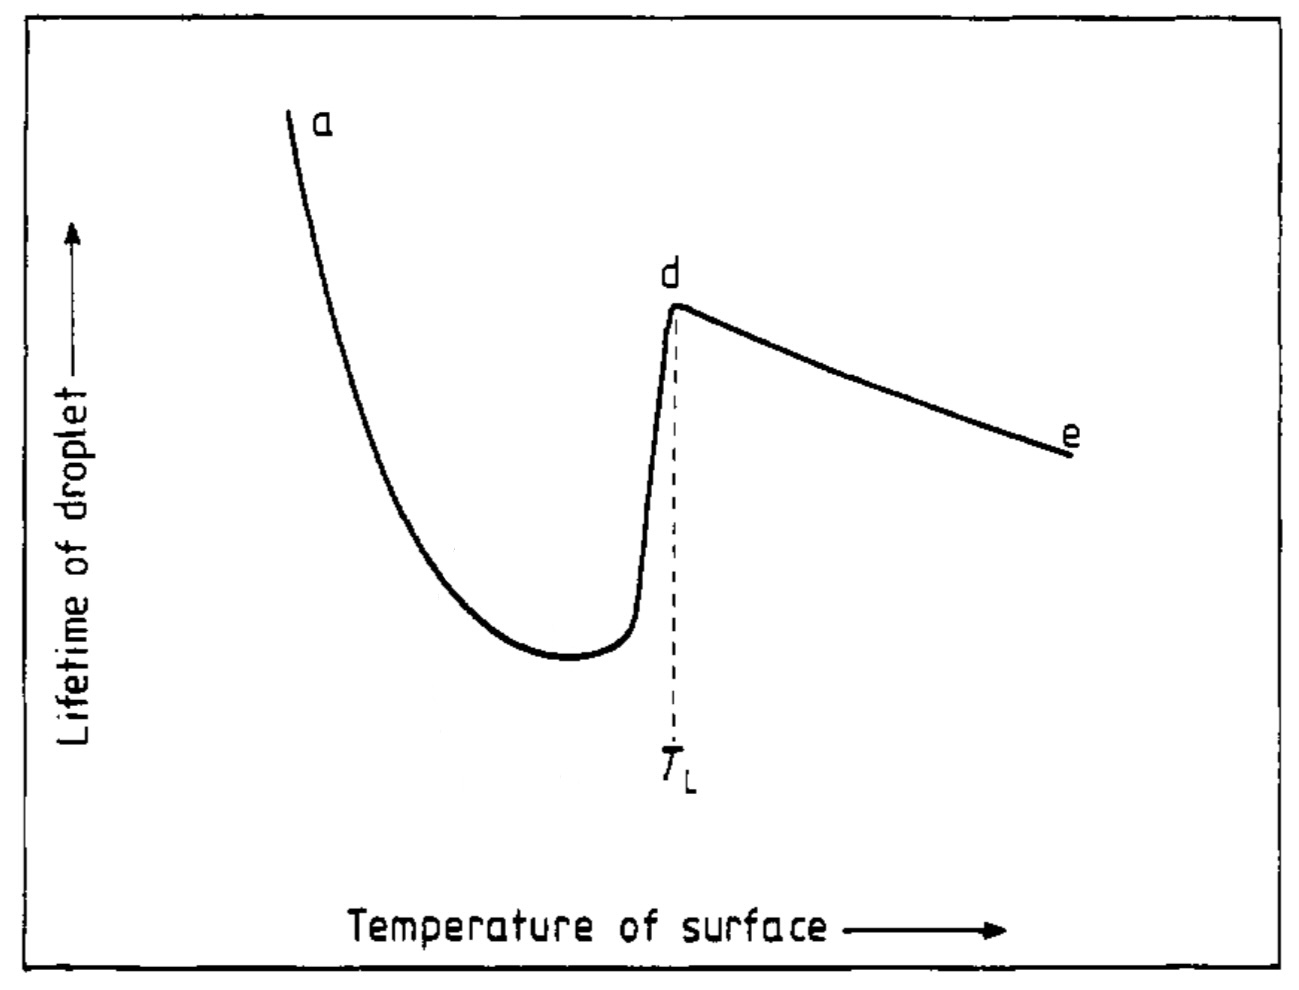
\includegraphics[scale = 0.14]{IMG_7600.jpg}}
\end{frame}

\begin{frame}{Полуэмперическое выражения для температуры Leidenfrost\ Point}
\textcolor[RGB]{0,128,255}{\sl Уравнение, полученное N.J. Baumeister and F.F. Simon (1973)}
\begin{doublespace}
\centering\[T_{LFP}=T_{f}+\frac{0.844T_{c}\left\{1-exp\left(-0.016\left[\frac{\left({\frac{p_{s}}{At}}\right)^{1.33}}{\sigma_{f}}\right]^{0.5}\right)\right\}-T_{f}}{exp\left(3.066\times10^6\beta\right)erfc\left(1758\sqrt{\beta}\right)} \ ,where\] 
\ \[\beta=\frac{1}{k_{s}p_{s}c_{p}}\  ,   \ \  \ T_{i}=\frac{{\left(kpc_{p}\right)_{s}}^{0.5}T_{s,0}+{\left(kpc_{p}\right)_{f}}^{0.5}T_{f,0}}{{\left(kpc_{p}\right)_{f}}^{0.5}+{\left(kpc_{p}\right)_{f}}^{0.5}}\] 
\end{doublespace}
\end{frame}
\begin{frame}{Графическое представление процесса}
\begin{figure}[h]
\centering
\center{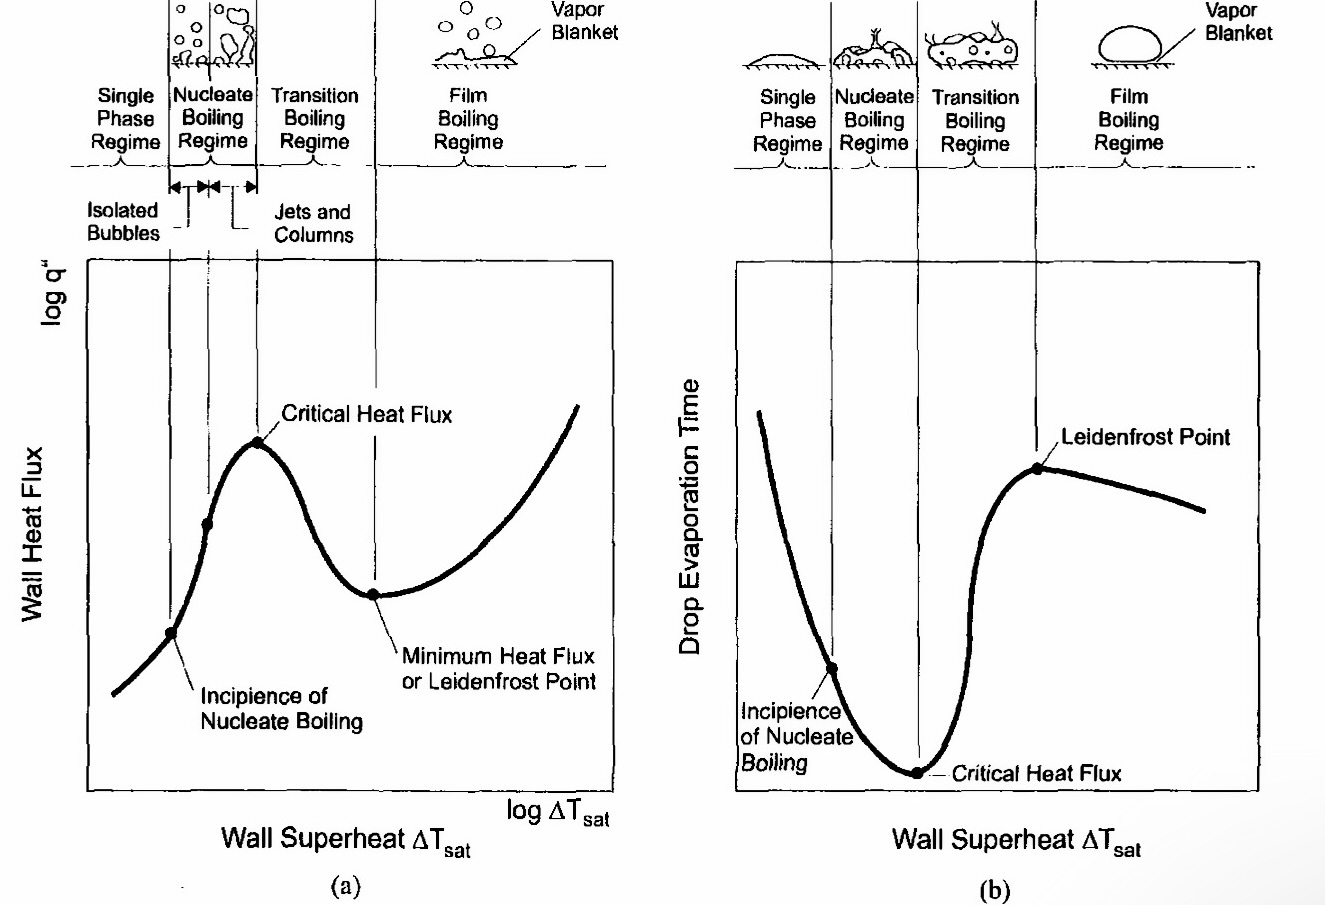
\includegraphics[scale=0.23]{299600A5-5ABD-41A7-B1D9-63D9061B2465_1_201_a.jpeg}}
\label{fig:image}
\end{figure}
\end{frame}

% Resultados
\include{tex/resultados/resultados}
\section{Experiment}
\begin{frame}{Графическое представление процесса}
\begin{minipage}[h]{0.49\linewidth}
\center{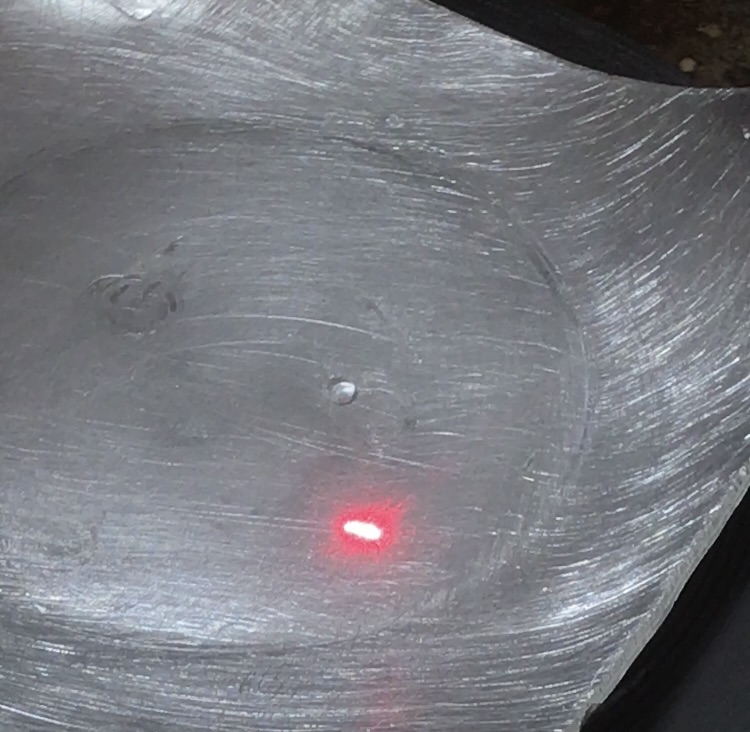
\includegraphics[width=\linewidth]{F4A34488-0441-48E3-91F2-E24B64D96CD6_1_201_a.jpeg}}
\label{fig:image}
\end{minipage}
\begin{minipage}[h]{0.49\linewidth}
\center{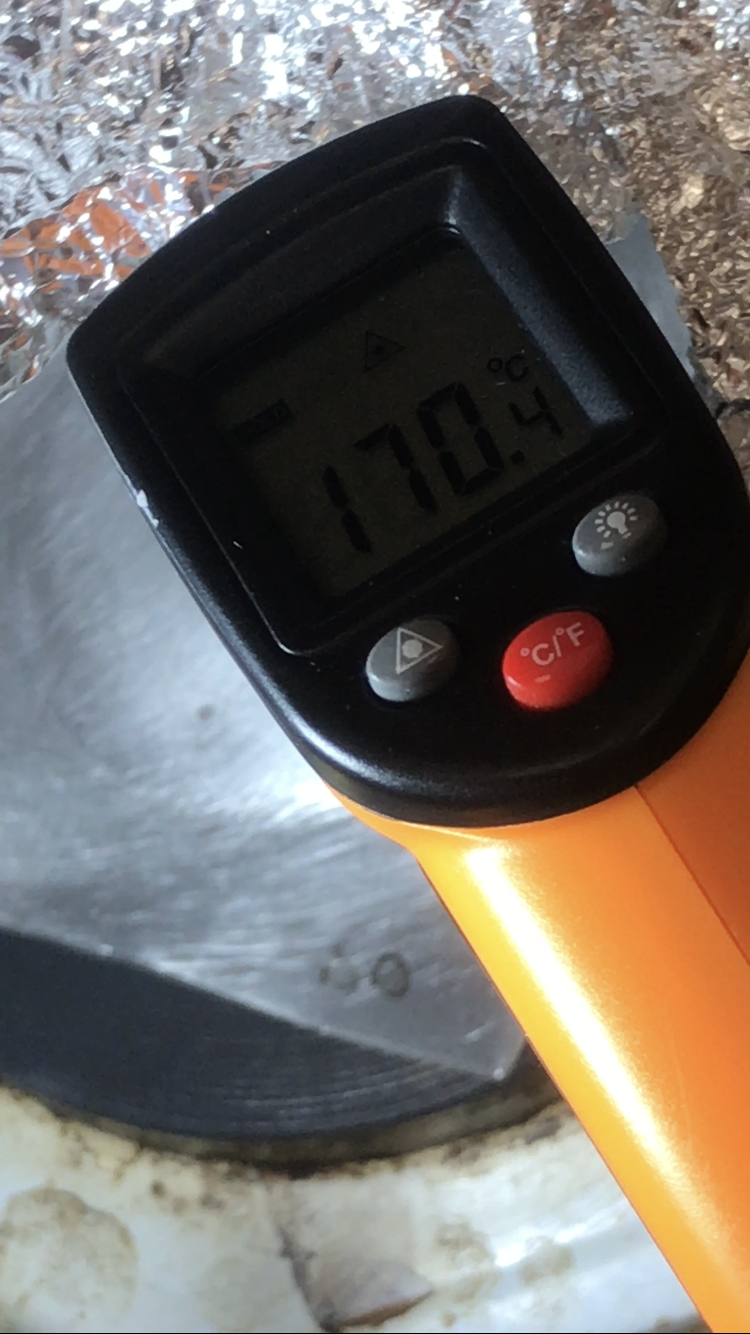
\includegraphics[width=0.8\linewidth]{IMG_1470.PNG}}
\end{minipage}
\end{frame}

\begin{frame}{Характиристики плёнки, теплообмен между твёрдым веществом и жидкостью, скорость испарения жидкости.}
\begin{block}{\sl Проводимоть в паровом зазоре - основоной механизм теплообмена между твёрдым и жидким}
Тепловой поток на единицу площади  \(k\frac{T_{S}-T_{B}}{b} = \frac{k\triangle T}{b}\), где \(\triangle T\) - разница температур между твёрдым веществом и температурой кимения жидкости k - теплопроводность пара.
\end{block}
Введём массу жидкости испаряющуюся за единицу времени \(\dot{M}\) после короткого времени, для возвращения значения температуры до \(T_{B}\), понадобится \(L\dot{M}\sim\left(\frac{k\triangle T}{b}\right)R^{2}\), L - теплота парообразования. Осталось определить b - толщину плёнки и \(\dot{M}\). Из рисунка ({b}) видно, что зазор (паровой слой) имеет размеры: несколько миллиметров в длине и 0,1 мм в толщине. Поэтому пар выходит с течением Пуазейля.
\end{frame}

\begin{frame}{}
\center{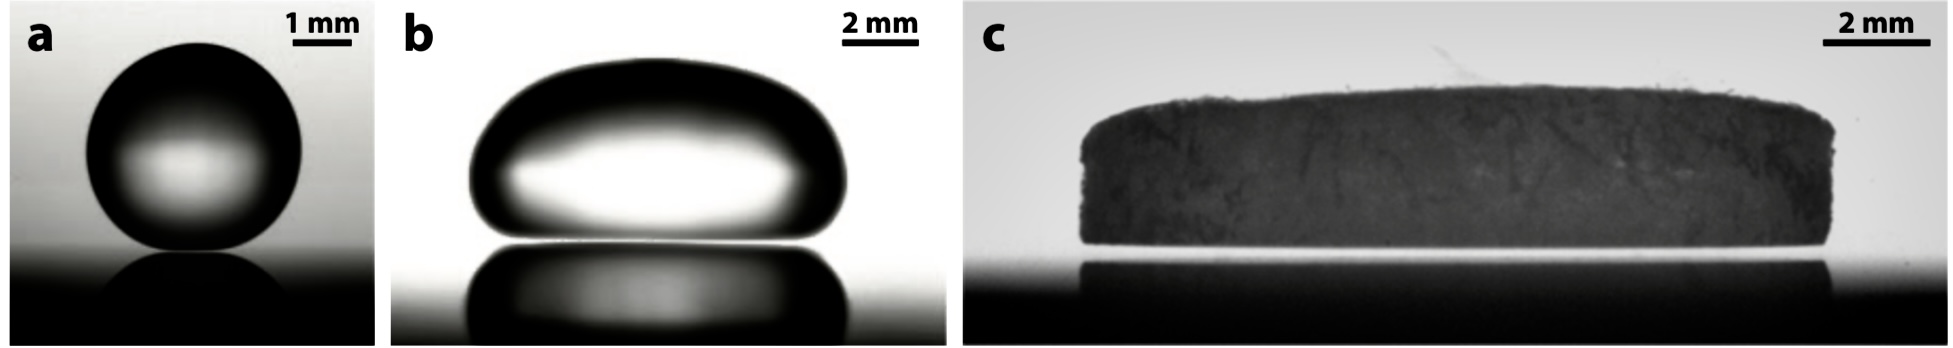
\includegraphics[width=\linewidth]{foto/IMG_7591.jpg}}
\begin{block}{\slВведём зависимость между потоком пара и градиетом давления:}
\(\dot{M}\sim\left(\frac{\rho_{\upsilon}Rb^{3}}{\eta_{\upsilon}}\right)\triangledown P\), где \(\rho_{\upsilon} и \eta_{\upsilon}\) - плотноть пара и вязкость, капля оказывает гидростатическое давление \(\rho g\iota_{c}\), откуда \(\dot{M}\sim\left(\frac{\rho_{\upsilon}b^{3}}{\eta_{\upsilon}}\right)\rho g\iota_{c}\), в стационарном режиме плёнка питается испарением капли со скоростью, с которой пар ускользает, что даёт закон для толщины плёнки \(b\sim\left(R\beta\right)^{1/2}\), где \(\beta = {\left(\frac{k\triangle T\eta_{\upsilon}}{L\rhoa_{\upsilon}\rhoa g\iota_{c}}\right)}^{1/2}\), подсчитав значения для b и подставляя их в формулу для \(\dot{M}\) мы получим значение пара, образованного в единицу времени.
\end{block}
\end{frame}

\begin{frame}{}
\begin{block}{\sl Итог:}
Предполагая, что капля испаряется только своим дном получим время жизни капель Лейденфроста: \(\tau=\frac{M}{\dot{M}}\). Если счиать, что время жизни мало, то формуля для теплопроводности будет упрощена и иметь вид: \( \dot{M} \sim \left(\frac{k \triangle T}{Lb}\right)R^{2} \sim \rho_{\upsilon}\dot{b}R^{2}\), в предположении что b должен зависить от времени как: \(\left(\frac{k\triangle Tt}{L\rho_{\upsilon}}\right)^{1/2}\)
\end{block}
\center{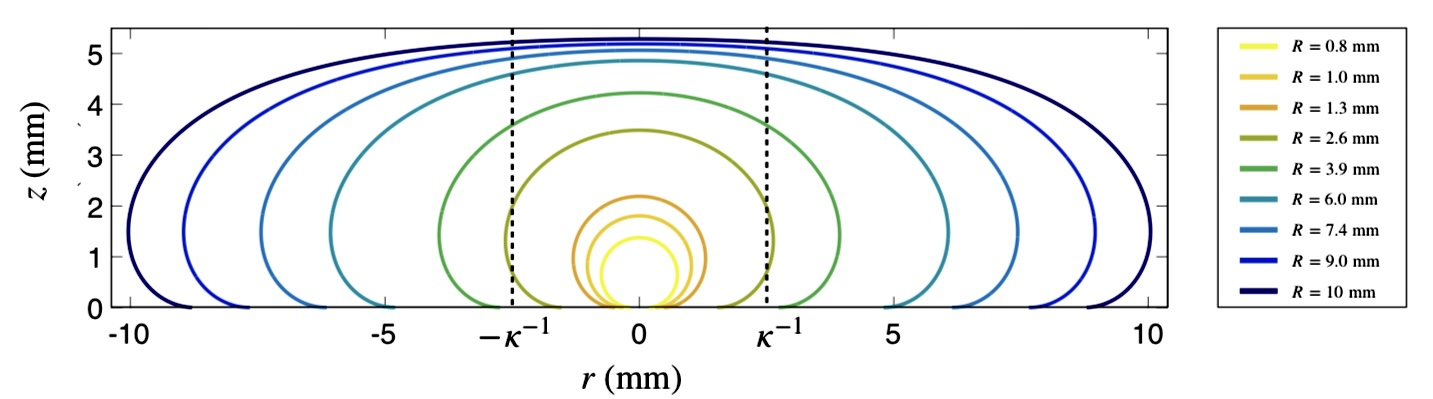
\includegraphics[width=\linewidth]{IMG_7597.jpg}}
\end{frame}

\begin{frame}{Установка}
\sidefig (0.5\linewidth)(0.5\linewidth) {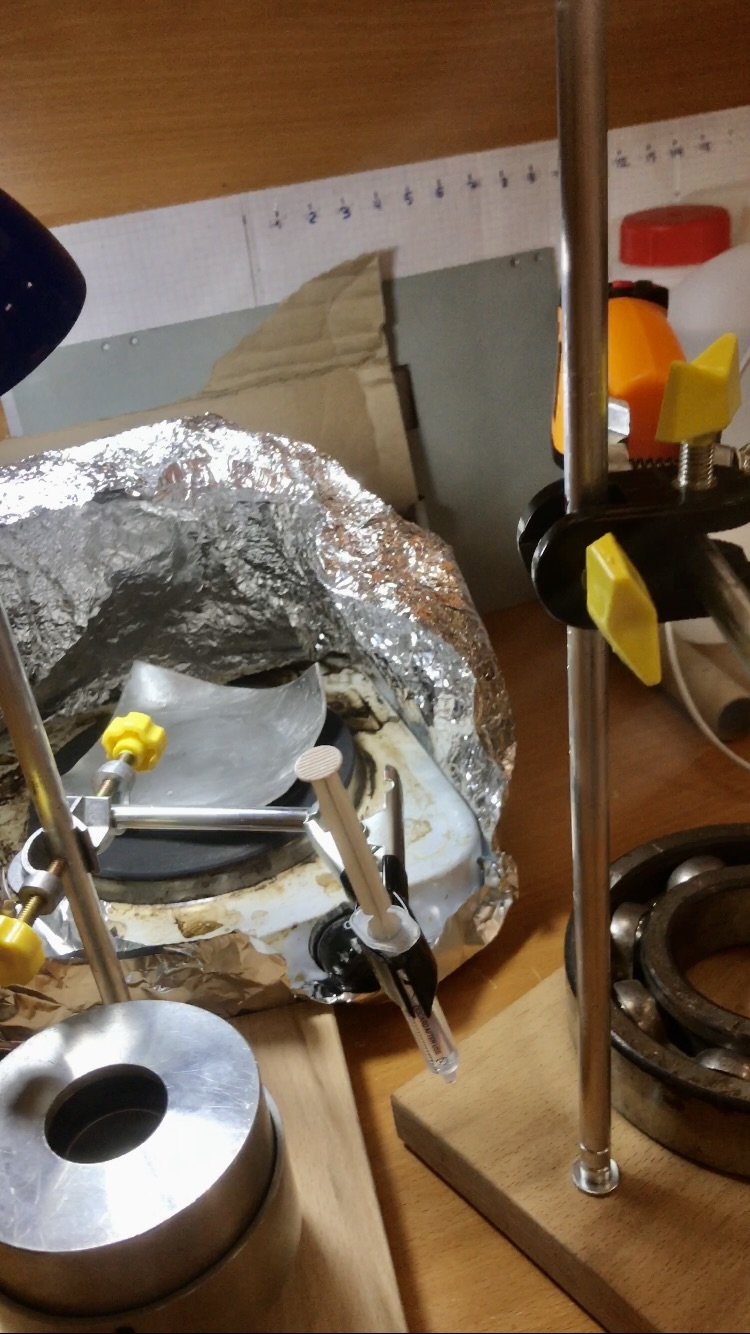
\includegraphics[scale=0.155]{97B356EC-468F-416D-9B06-919921896A27_1_201_a.jpeg}}{В установке пришлось использовать \textcolor[RGB]{0,128,255}{\sl два штатива}, для фиксации \textcolor[RGB]{0,128,255}{\sl лазерного термометра и шприца с дистилированой водой}, с целью не изменять их наклон и высоту во воремя эксперемента, а так же, чтобы изолировать систему от ветра и конвекционных потоков, использовали \textcolor[RGB]{0,128,255}{\sl защитную конструкцию из фальги}. Нагревали, \textcolor[RGB]{0,128,255}{\sl отшлифованную алюминиевую пластину}, в которой сделали углубления для удержания капли на месте.}

\end{frame}

\begin{frame}{}
\sidefig (0.5\linewidth)(0.5\linewidth)
{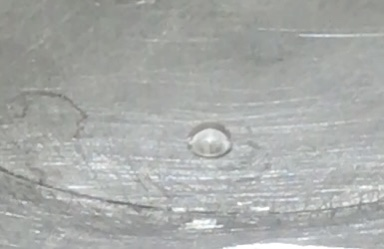
\includegraphics[scale=0.35]{5F8D7E02-0952-4090-83E1-37FAFF303F95_4_5005_c.jpeg}}{\vspace{0.10cm}Измерение проводились в пределах от 220\(C^{\circ}\) до 50 \(C^{\circ}\). Капали с помощью щприца, для чего провели предварительное измерение капель, с помощью весов, добившись одинаковые значения для масс капель, настроив установку, получили среднее}
\sidefig (0.5\linewidth)(0.5\linewidth)
{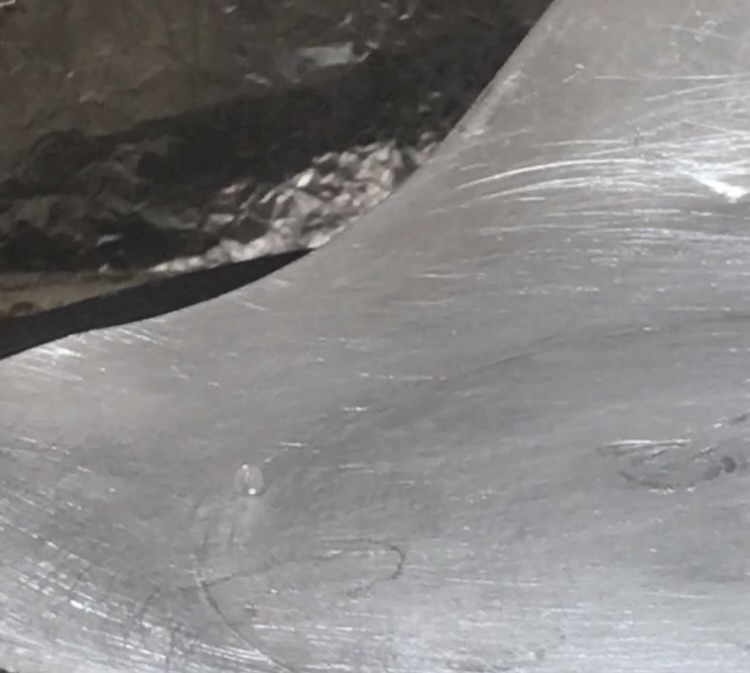
\includegraphics[scale=0.18]{A82B7535-E316-43B4-BE76-A6D4F11E907F_1_201_a.jpeg}}{значения для массы капли:\\
\[\overline{M} = 0,042 \pm 0,001 g. \]
Шприц, мы отворачивали и поворачивали обратно, чтобы избежать нагрева воды, так как капать необходимо было с минимальной высоты}
\end{frame}
% Conclusao
\section{Data processing}
\begin{frame}{Graph}
\center{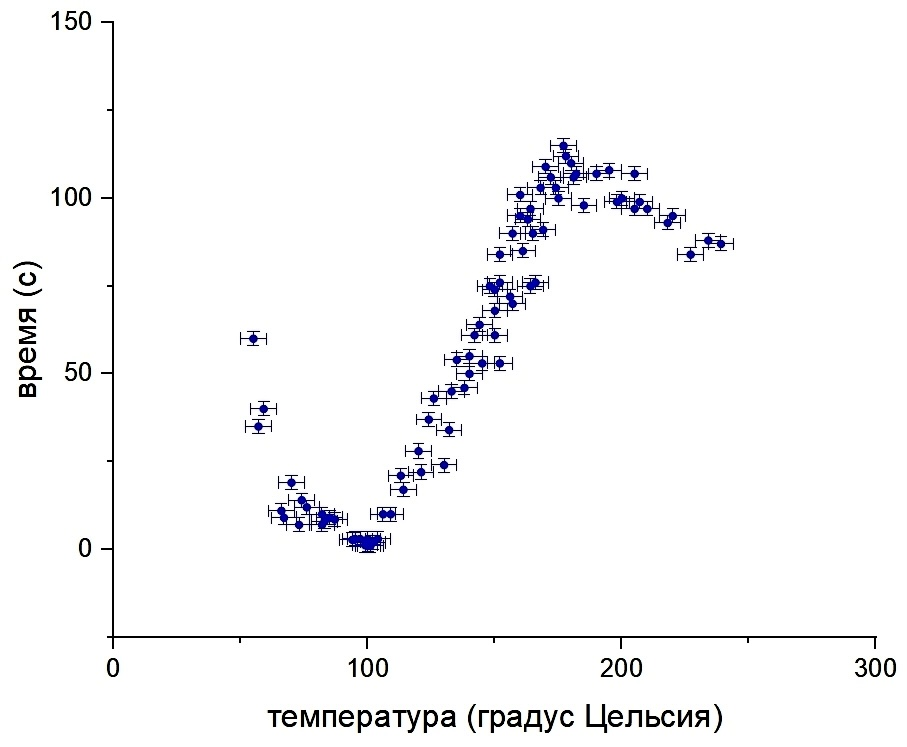
\includegraphics[scale = 0.28]{tex/conclusao/IMG_7656.jpg}}
\end{frame}

\begin{frame}{Graph approximation}
\center{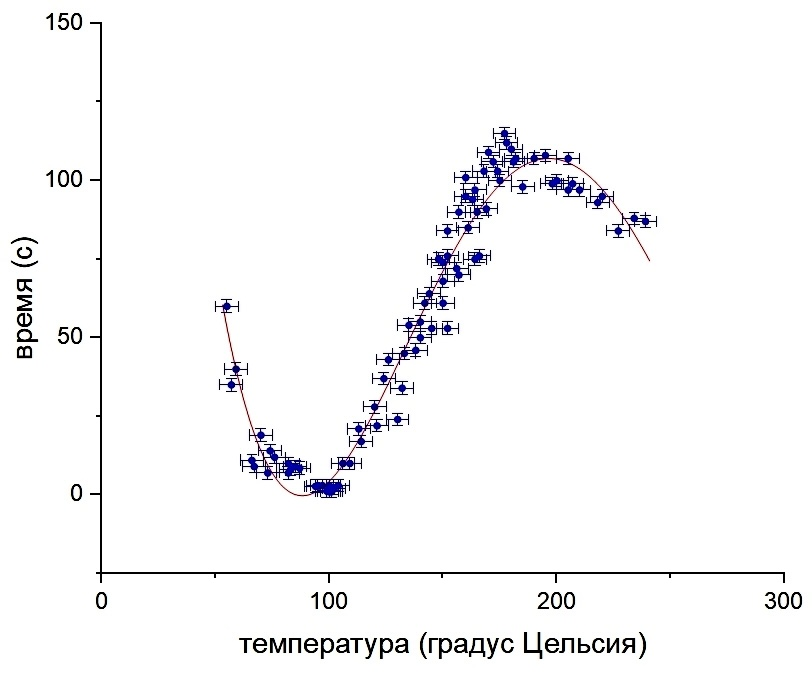
\includegraphics[scale = 0.3]{tex/conclusao/IMG_7596.jpg}}
\end{frame}
 \begin{frame}{Немного наблюдений, обнаруженных во время эксперемента}
  \begin{block}{Геометрия капли}
   После падения даже с небольшой высоты, у капли самовозбуждаются колебания, которые затухают без внешнего воздействия, с уменьшением размера капли. 
  \end{block}   
  \center{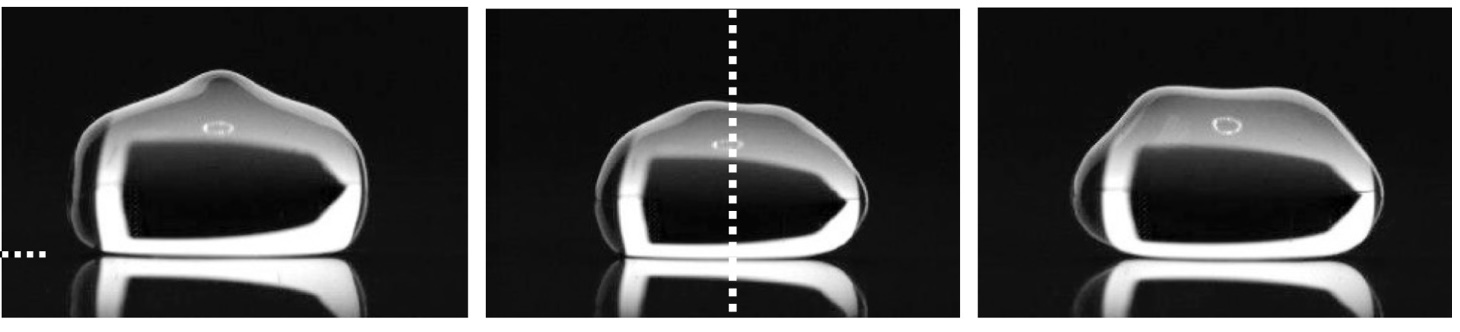
\includegraphics[scale = 0.2]{tex/conclusao/IMG_7594.jpg}}
  \begin{block}{}
      Такая нестабильность является обратной нестабильностью Рэлея-Тейлора, которая происходит, когда сила гравитации преобладает над поверхностным натяжением.
  \end{block}
 \end{frame}

\begin{frame}{}
  \begin{minipage}[h]{0.49\linewidth}
{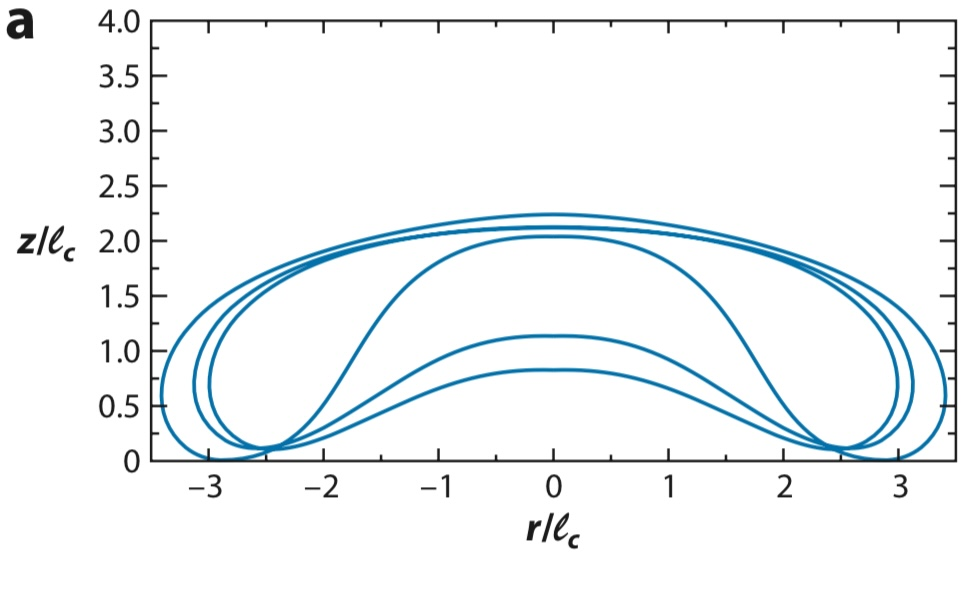
\includegraphics[width=\linewidth]{tex/conclusao/IMG_7593.jpg}}
\label{fig:image}
\end{minipage}
\begin{minipage}[h]{0.49\linewidth}
{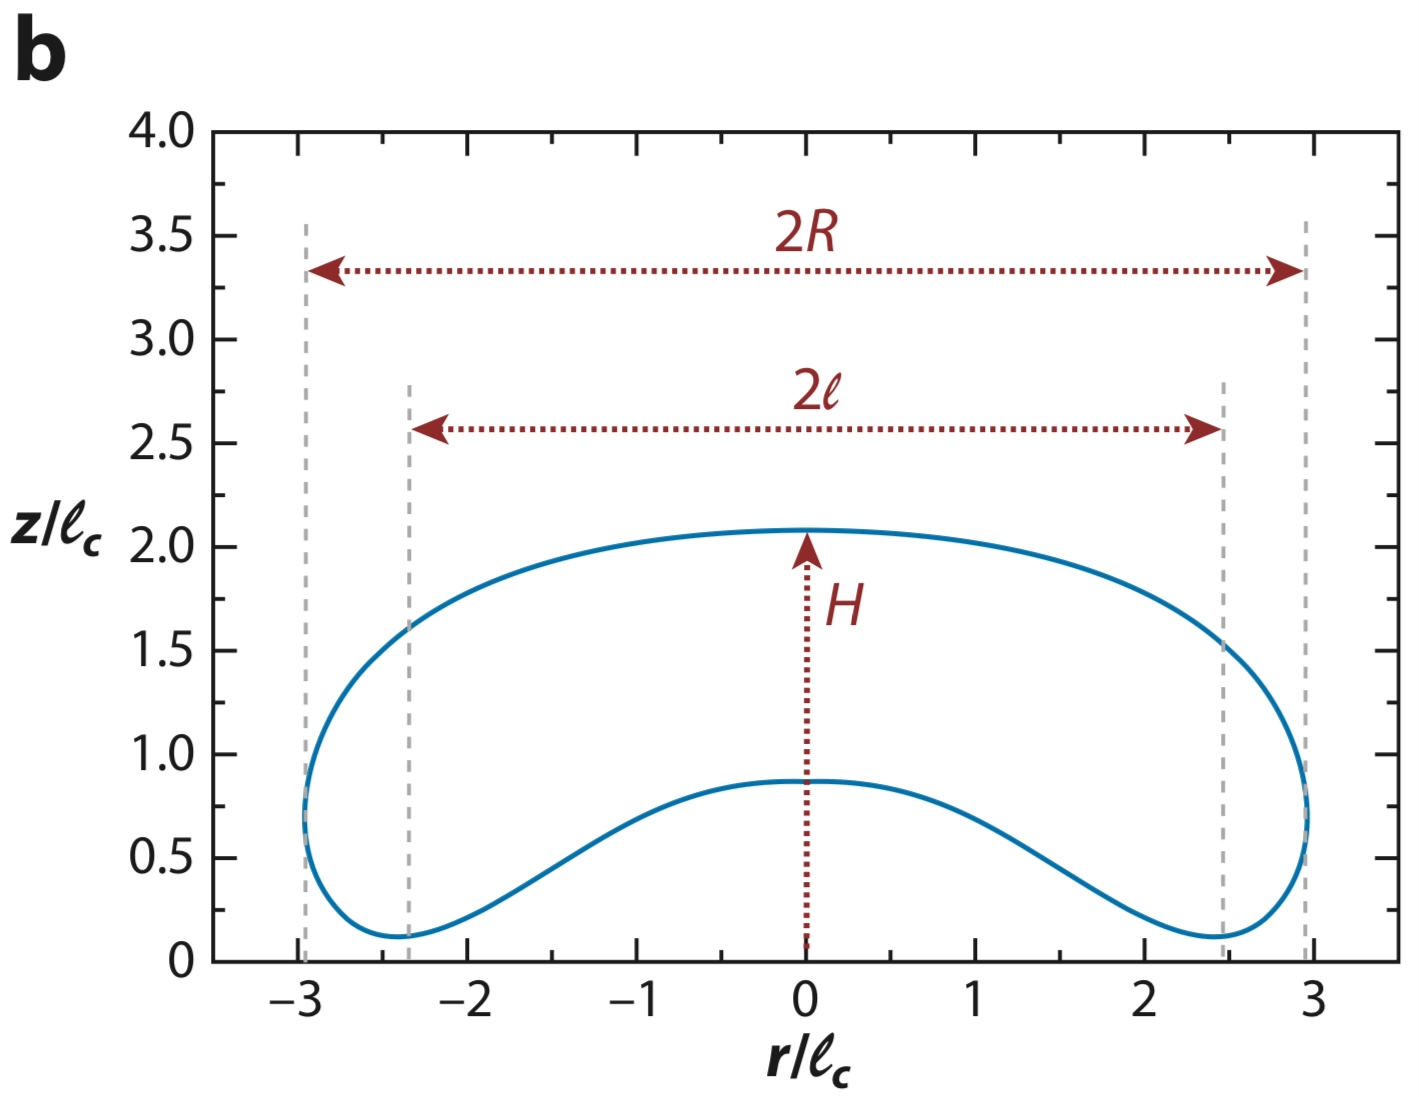
\includegraphics[width=\linewidth]{tex/conclusao/IMG_7592.jpg}}
\end{minipage}
\begin{block}{Зависимость от радиуса}
 Неравновесие сил происходит, когда радиус контакта \(\ell\) превышает порог \(\ell^{*} = 3\ell_{c}\), определяется, как длина капиляра, соответсвующий критический радиус \(R^{*}=4,3\ell_{c} \), где
 \({\ell_{c}=\left(\frac{\gamma}{\rho g}\right)}^{1/2}\), \(\gamma=59\ mN\ m^{-1}\), - коэфициент поверхностного \\
 \vspace{0.10cm}
 натяжения \(\ell_{c}=2,5 mm.\) для воды.
 \end{block}
\end{frame}

 \begin{frame}{}
 \vspace{0.2cm}
   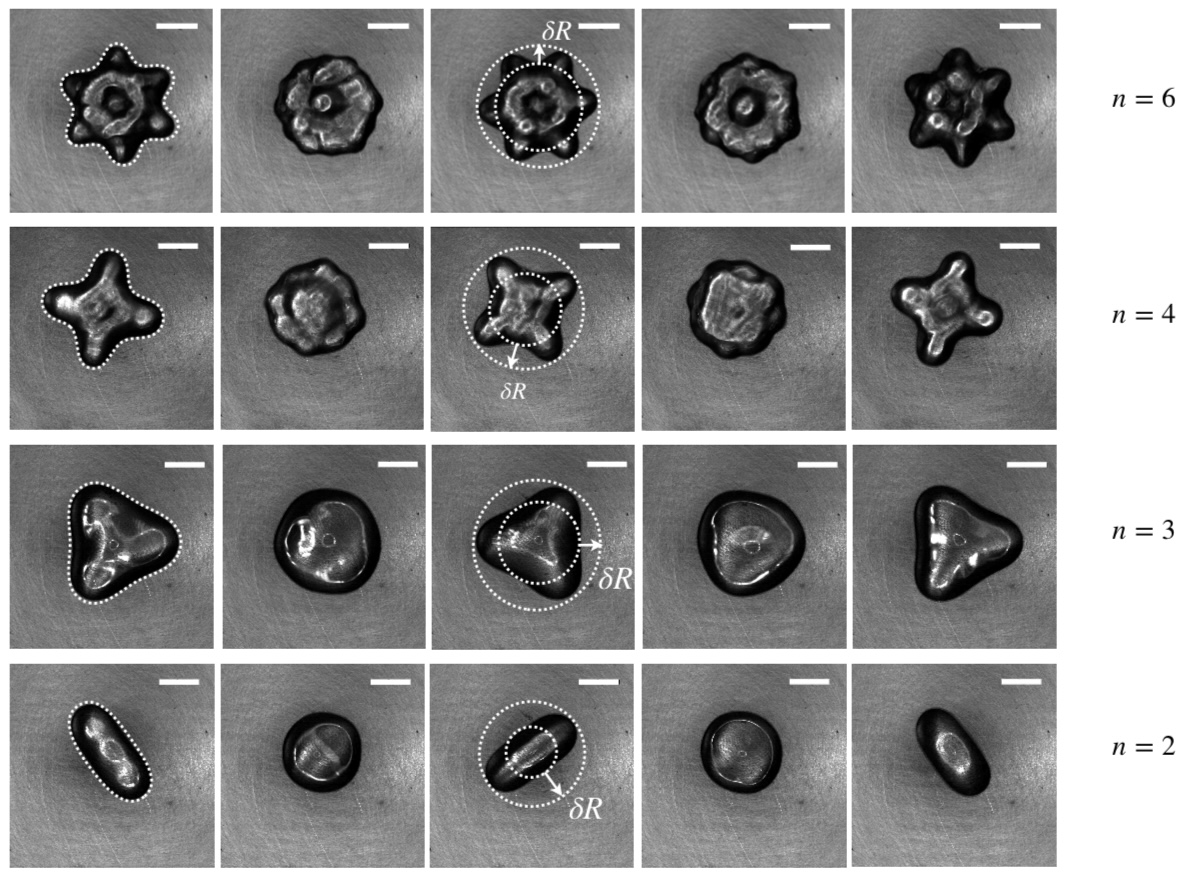
\includegraphics[width=\linewidth]{tex/conclusao/IMG_7598.jpg}
 \end{frame}
 \begin{frame}{}
 \vspace{1.5cm}
 \begin{block}{Как описать, явления на картинках, с разными рисунками, пр. разных n?}
 Осесиметричное сферическое падение подвергается свободным колебаниям на естественной резонансной частоте \(f_{n}\), где n - целые числа, в пределах малых деформаций задаётся уравнением:
 \[f_{n}= \frac{1}{2\pi}\sqrt{n\left(n-1\right)\left(n+2\right)}\sqrt{\frac{\gamma}{\rho R^{3}}}\]
  
 \end{block}
 \end{frame}
% Referencias
\section{Сonclusion}
\begin{frame}{Сonclusion}
\begin{block}{Феномен Leidenfrost Effect содержит многие аспекты межфазной гидродинамики.}
\begin{itemize}
    \item Именно в этом процессе осуществляются явления низкого трения между двумя поверхностями.
    \item низкий уровень теплопроводности, что позволяет удерживать температуру в нужных пределах.
    \item наличие плёнки поверх горячей поверхности позволяет использовать данные методы в закалке и охлаждении стержней в атомных электростанциях.
\end{itemize}
\end{block}
	\bibliography{bib/bibliografia}
\end{frame}
% Agradecimentos
\section{Сompletion}
\begin{frame}{Сompletion}
\vspace{2.1cm}
\begin{block}{}
	\large \color{navy} \textbf{\sl В завершении, мы сняли видео, в котором смогли запечатлить, как рассказанные аспекты, так и карасивые явления.}
\end{block}

\includegraphics[scale=0.07]{kisspng-video-clip-art-simple-blue-play-button-design-5a7be6707c3509.5341037115180693605088.png}
\end{frame}
\end{document}